\documentclass[a4paper,12pt,twoside]{book}

%--------------------------------------------------------------------------
%Packages
%--------------------------------------------------------------------------
\usepackage{amsfonts,amsmath,amssymb}
%\usepackage{amsthm}
\usepackage{xspace}
\usepackage{fancyhdr}
%\usepackage{pythonhighlight}
\usepackage{listings}
\usepackage{color}
%\usepackage{these}
\usepackage{textcomp} % for degrees : command \textcelsius also \textangle for angles

%\usepackage{epsf}
\usepackage[bookmarks=true,pdftex,colorlinks=true,urlcolor=blue,pdfstartview=FitH]{hyperref}
  \pdfcompresslevel=9
  \hypersetup{
    pdftitle={Practical course reader on control of part},
    pdfauthor={A. de La Fortelle},
    pdfsubject={HDR},
    pdfkeywords={ITS}
  }
\usepackage[pdftex]{graphicx}
\DeclareGraphicsExtensions{.jpg,.mps,.pdf,.png} % Formats d'images
\graphicspath{{Figures/}} % Chemin vers les figures



%----------begin commands----------
\newcommand{\ud}{\mathrm d} %COMMENT: for infinitesimal dx = \ud x and dy = \ud y TODO: DO YOURSELF all replacement
\renewcommand\theequation{\arabic{equation}}
\renewcommand{\figurename}{Fig.}
\newcommand{\subgroup}[2]{\medskip \emph{Prepared by subgroup #1 (#2)}\medskip}
%----------end commands----------

%----------begin style---------------
\lstloadlanguages{Matlab, Python}
 
\definecolor{codegreen}{rgb}{0,0.6,0}
\definecolor{codegray}{rgb}{0.5,0.5,0.5}
\definecolor{codepurple}{rgb}{0.58,0,0.82}
\definecolor{backcolour}{rgb}{0.95,0.95,0.95}

\lstdefinestyle{codestyle}{
    basicstyle=\small\ttfamily, 
    backgroundcolor=\color{backcolour},   
    commentstyle=\color{codegreen},
    keywordstyle=\color{blue},
    numberstyle=\tiny\color{codegray},
    stringstyle=\color{codepurple},
    basicstyle=\footnotesize,
    breakatwhitespace=false,         
    breaklines=true,                 
    captionpos=t,                    
    keepspaces=true,                 
    numbers=left,                    
    numbersep=5pt,                  
    showspaces=false,                
    showstringspaces=false,
    showtabs=false,                  
    tabsize=2
}

\lstset{style=codestyle}
%---------end style----------------


%--------------------------------------------------------------------------
%Document
%--------------------------------------------------------------------------
\begin{document}
\frontmatter
\thispagestyle{empty}
\topmargin -5mm
%\textheight 25cm
%\enlargethispage{4cm}
\headsep 0cm
\font\tensmc=cmcsc10 scaled 1200
%\font\grand=cmbx12 scaled 3000
\font\grand=cmbx12 scaled 1600
\font\moyen=cmbx12 scaled 1200

\noindent
Version: \today
%version finale du \today.


\vskip 1cm

%\centerline{.}
%\centerline{\rule{\textwidth}{2mm}}
\begin{center}
{\grand  Practical Course Reader

\bigskip for Control of distributed systems}

\vspace{2cm}
{        made at the}\bigskip

{\moyen  University of California at Berkeley} \medskip

\vskip 0.8 cm
{\tensmc by \moyen Arnaud de LA FORTELLE}
\vskip 0.8 cm
{\moyen  visiting professor from MINES ParisTech} \medskip


%\vskip .4cm
\vfill
\centerline{\hbox to 3cm{\leaders\hrule\hfil}}
\vskip .3cm
\smallskip

{\moyen for the course CE-C291F --- EE-C291 --- ME-C236}

\smallskip
\smallskip
\centerline{\hbox to 3cm{\leaders\hrule\hfil}}
\end{center}
\vskip 0.5cm plus 0.6cm



\vfill
With the help of:
\begin{center}
\begin{tabular}{lll}
%MM. & {\bf Bradley Cage} & student\\
& {\bf Bradley Cage} & student\\
& {\bf Hongbei Chen } & student\\
& {\bf Yue Hu } & student \\
& {\bf Carlin Liao} & student\\
& {\bf Xin Peng} & student\\
& {\bf Robert Ruigrok } & student\\
& {\bf Lin Yang} & student\\
& {\bf Qingan Zhao } & student\\
& {\bf Ruitong Zhu } & student
 %\phantom
\end{tabular}
\end{center}

%\centerline{--\ 2000\ --}

\newpage

\pagestyle{fancy}
\addtolength{\headsep}{\marginparsep}
\addtolength{\headheight}{\baselineskip}
%\addtolength{\headwidth}{\marginparsep}
%\addtolength{\headwidth}{\marginparwidth}
%\renewcommand{\chaptermark}[1]{\markboth{#1}{#1}} % remember chapter title
%\renewcommand{\sectionmark}[1]{\markright{\thesection\ #1}}
\renewcommand{\chaptermark}[1]{\markboth{\thepart~~Ch.~\thechapter\ \ #1}{#1}}
\renewcommand{\sectionmark}[1]{\markright{\thesection\ #1}}
\fancyhf{}
%\fancyhead[LE,RO]{\bfseries\thepage}
\fancyhead[LE,RO]{\thepage}
\fancyhead[LO]{\small \sc \rightmark}
\fancyhead[RE]{\small \sc \leftmark}
\fancypagestyle{plain}{
\fancyhead{}
\renewcommand{\headrulewidth}{0pt}
}




%\href{Table of contents}{}
\tableofcontents
\addcontentsline{toc}{chapter}{Table of Contents}

%\listoffigures

\mainmatter

\thispagestyle{empty}
%----------------------------------------------------------------------
\chapter{Introduction}
\label{introduction.chap}
%----------------------------------------------------------------------

\section{Objectives}
%----------------------------------------------------------------------

This practical course reader aims at giving good advice to students realizing a project. Starting with the theoretical knowledge contained in the reader of Prof. Alexandre Bayen, students have to realize a project based on a distributed parameter system that they should:
\begin{enumerate}
	\item describe
	\item model
	\item explain
\end{enumerate}
The first part is a descriptive (i.e. qualitative) description of the system to be studied, its interest and the goal of the study. The second part is an elaboration, under simplifications, of a quantitative model (meaning here some kind of Partial Differential Equation and some control or optimization). The third part is an analysis of this model, either by solving the equations, by simulation or by a combination of both, using the tools learned during the course. It should lead to a better understanding of how the system works and how it can be optimized or controlled to fulfill the goals set in the description.

Therefore this practical course reader shows examples of modeling and various analysis methods that can support the creativity of the students realizing a project.

\section{System description}\label{description.sec}
%----------------------------------------------------------------------
A system is, according to Cambridge dictionary ``a set of connected things or devices that operate together''. There is no recipe to describe a system. However, it is often useful, instead of having an \emph{analytical} description (i.e. tear the system into pieces), to have a \emph{synthetic} one (i.e. seeking for a global view). Without any generalization, again, one can look after the following 4 views of a system:
\begin{enumerate}
	\item objective
	\item environment
	\item actions
	\item transformations
\end{enumerate}
One can very arguably contest these words, but remember they are only guidelines. In most systems, since they are man-made, there is a goal. This \emph{objective} is important to describe since it contains the meaning: what is it for? Note this is quite often the opposite of the analytical view: how does it work? However, in our case, this goal contains the information about the \emph{objective function} for optimization or for control. The \emph{environment} dictates what the system has to do: a system is never isolated and its goal is often closely related to its environment. At least, the \emph{actions} a system perform are partially internal and partially external, so that taking into account the environment allow understanding of disturbances but also the objective. Since a system is usually complex, it may evolve (i.e. experience \emph{transformations}) according to actions and in line with the objective. One can also think of transformation as internal states of a finite automaton.

In any case, a description is intended at telling the whole story to other people and this is why it is highly recommended to use only words, no formula, but drawings can well replace a thousand words.

\section{System modeling}
%----------------------------------------------------------------------
While a system description is intended to be purely qualitative, modeling aims at estimating some quantities. Very clearly, the choice of the quantities is decisive. Important quantities can be derived from the system description, such as the objective function (what to maximize or minimize?), the transformations (internal states) or environment variables.

There are many ways to measure quantities, e.g. numbers of vehicles in a microscopic view may be equivalent to measuring densities of vehicle at a macroscopic scale. Unfortunately there is no algorithm to produce significant model and this is a knowledge that needs practice. However, in our present case, namely partial differential equations modeling, there is very often a kind of scaling that is necessary in order to produce continuous-space and continuous time variables. Since this reader aims at being practical, the reader is referred to Chapter~\ref{modeling.chap} for modeling examples.

One can (too?) quickly summarize some usual quantities of interest:
\begin{itemize}
	\item macroscopic quantities (temperature, density, deformation...);
	\item variables (state space, time...) and parameters including the control;
	\item optimization criteria;
	\item invariant quantities (mass, energy, momentum...) and constraints;
	\item initial and boundary conditions.
\end{itemize}


\section{System explanation}
%----------------------------------------------------------------------
What is called here explanation has been also called ``solution'' during the course. It consists mainly in studying the model under various views and to produce new knowledge. This usually implies simulations, analytical analysis, optimization and visualization; all previous methods can be compared or combined in order to give more insight of the model.

\subsection{Analysis}\label{analysis.sec}
Analysis is important for the concepts it carries. We have learned a few methods to exactly solve or to transform the PDEs:
\begin{enumerate}
	\item Dimensional analysis allow to build interesting quantities that should remain constant;
	\item Product-form solutions leads to decomposition of solutions (often in the type of Fourrier transform) with knowledge of the modes and their frequencies (spatial and temporal).
	\item the method of characteristics is a powerful methods to build solutions, even discontinuous like shockwaves in LWR equations. The characteristic curves are interesting features.
\end{enumerate}
In the present course, students should perform some initial analytical analysis, even if it does not lead to a complete solution, in order to exhibits interesting quantities as mentioned above. These quantities should be used as guidelines as far as possible for further study.

\subsection{Simulation}\label{simulation.sec}
Simulation is interesting for all the data it brings. However there are many ways to simulate a system. At least we can mention:
\begin{itemize}
	\item Microscopic simulation --- often agent-based --- where a lot of microscopic entities evolves with their dynamics; This method is relevant when the PDE is a macroscopic view of the system, i.e. when it is derived from a scaling;
	\item Finite differences schemes, that is often a direct implementation of the dynamics underlying the PDE (differences apply on a discretization of space and time);
	\item Finite elements is usually associated to computation of eigenvalues and eigenvectors, i.e. to product-form solutions and the computation of modes; in this case, discretization is made through a projection of the functions onto a finite (functional) basis.
\end{itemize}
In this course, students have to produce simulations. The goal is to exploit the data to visualize the system evolution (see also Section~\ref{visualization.sec}) and get a better understanding. One of the main problem of simulation is to have a clear idea of the quantities to be displayed, be it statistics, metrics or functions. This is why a good prior analysis (see also Section~\ref{analysis.sec}) is a good idea. A must in simulation is to compare quantities computed from the output of the simulation with similar quantities computed from theoretical analysis: e.g. number of vehicles per km in micro-simulation with densities in LWR equations.


\subsection{Optimization or control}\label{optimization.sec}
The goal of this course is to learn how a system can be controlled or optimized. This requires to have a good description of the system in order to have clear ideas of what is to be optimized or controlled. Usually, the design of the control is free and this is where students can be creative.

There is a very common distinction between 2 close concepts: planning and control. In most real systems, the planning phase is responsible for building suitable a path, according to the dynamics of the system and to the environment; then, a control loop ensures the systems follows this path by using actuators (the controls) and taking care of disturbances (in sensors and in actuators). Planning is open-loop, usually with a simple model (deterministic...) but with a complex cost function that expresses the desirable behavior. Control is closed-loop, designed to be robust, taking into account noises and disturbances, with a simple cost function: follow the plan.

Techniques are very diverse and really depend on the system and the kind of control. Examples are given in Chapter~\ref{control.chap}.

\subsection{Visualization}\label{visualization.sec}
The visualization aspect of a study may be the most important yet the most challenging. Indeed, a drawing is extremely instructive, provided it is well explained. But the beauty can be misleading and the students have to take great care of the quantities they illustrate: What should be seen in the drawing? What does it tell us? Does it compare well with existing knowledge or not?

Therefore it is advised to start quickly (very early with simulation data) to try to see something and to continuously improve the visualization aspect. It is important for explaining the results as well as for enhancing the students' own understanding (and debugging the codes, very often).

\thispagestyle{empty}
%----------------------------------------------------------------------
\chapter{Modeling}
\label{modeling.chap}
%----------------------------------------------------------------------

\section{Objectives}
%----------------------------------------------------------------------

\section{Derivation of partial differential equations}
%----------------------------------------------------------------------

\subsection{2D wave equation}
% ***********************************************************************************
% Pure LaTeX part to be inserted in a document (be careful of depencies of packages & commands
% Prepared by XXX and YYY under the supervision of Arnaud de La Fortelle
% Fall 2017
% 2D wave propagation subsection of the modeling part
% ***********************************************************************************

\subgroup{1}{Bradley Cage and Lin Yang}

\paragraph{Description}
\begin{figure}[htb]
	\centering
	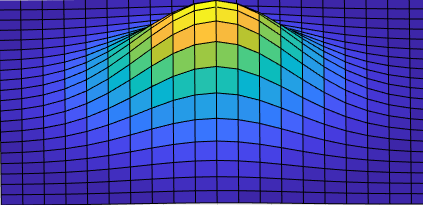
\includegraphics[width=10cm]{Figures/2D_waves_system.png}       
	\caption{The membrane system }
	\label{2D_waves_system.fig}
\end{figure}

Our system is comprised of a flexible membrane stretched to some shape, with all of its edges fixed in place. The desired goal is to understand the vertical position of the various points on the membrane over time. The membrane in this system has vertical deflections which are small compared to its overall size, and deflections happen only in the vertical direction.

This 2D system is a continuation of the 1D wave equation, and is a natural precursor to the 3D wave case. 


\paragraph{Model}
Assumptions:
\begin{itemize}
	\item Membrane has uniform planar density $\rho$
    \item The tension per unit length, $F_t$, caused by stretching the membrane is the same at all points and in all directions and does not change during the motion
    \item Vertical position is given by some function $u(x,y,t)$
\end{itemize}
\begin{figure}[htb]
	\centering
	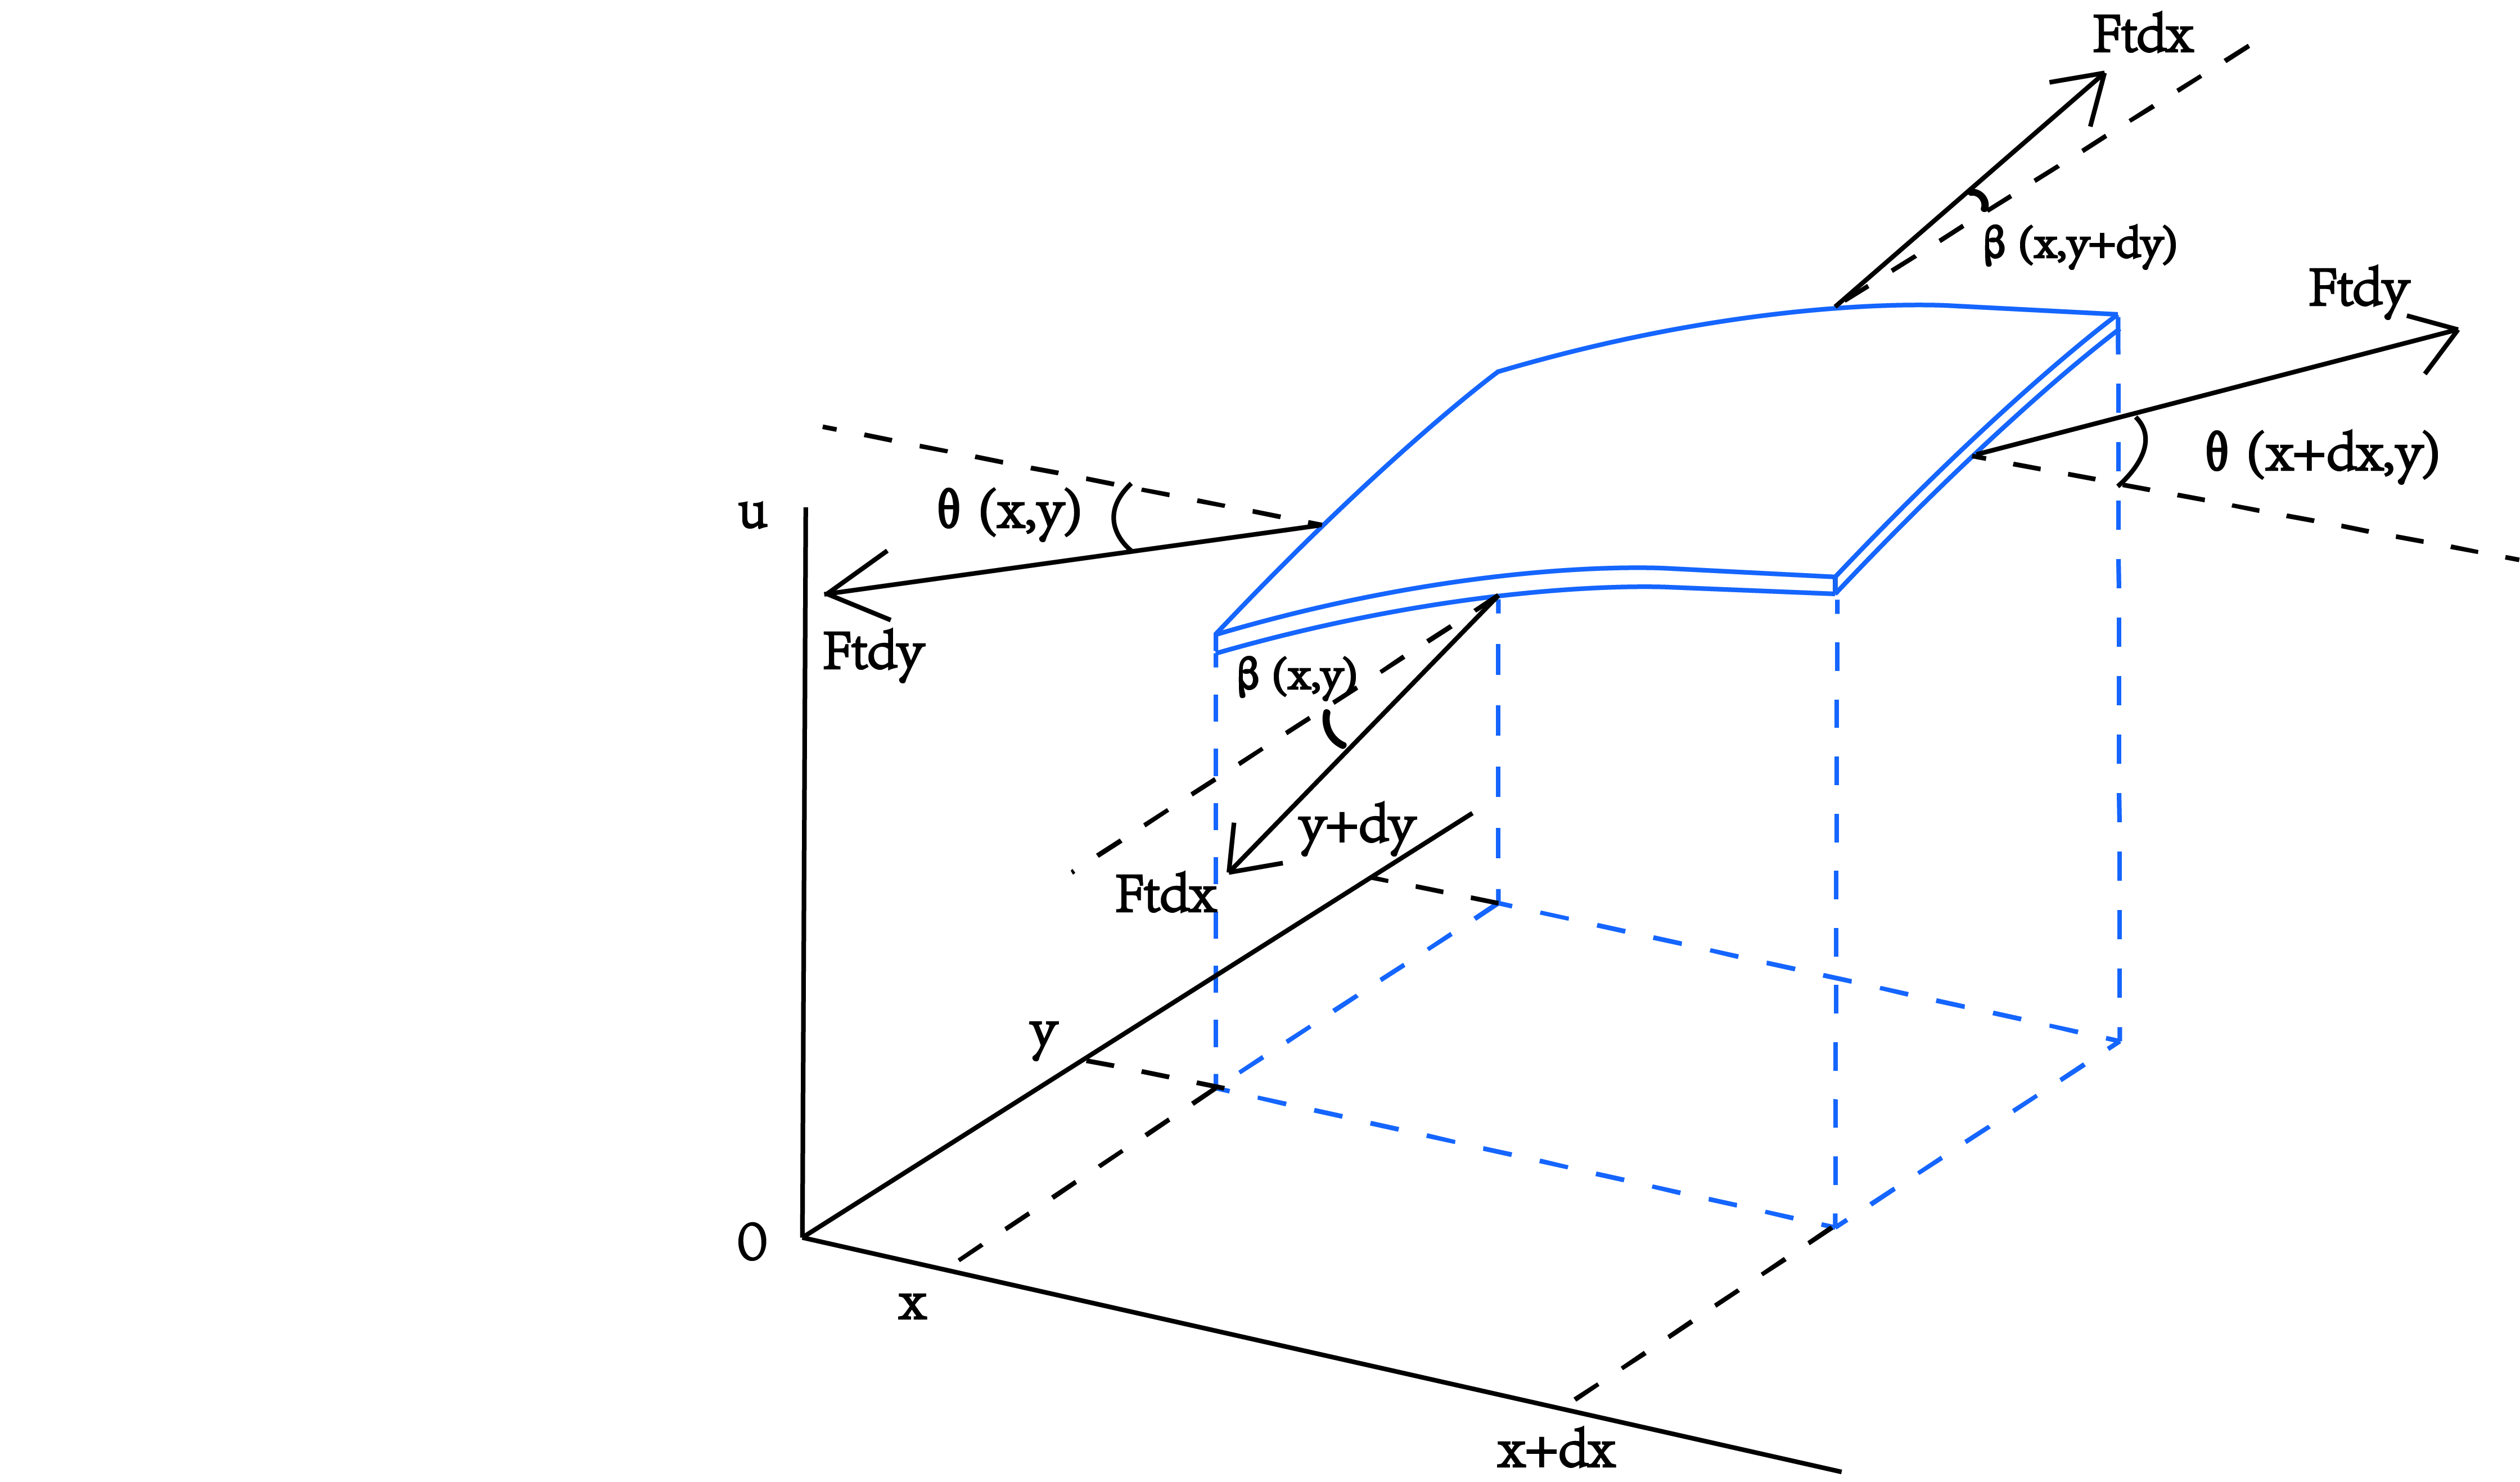
\includegraphics[width=15cm]{Figures/2D_waves_model.png}       
	\caption{The force analysis of a small section of the membrane system }
	\label{2D_waves_model.fig}
\end{figure}
We begin from basic principles.

$$\Sigma F = m\vec{a}$$

\noindent Taking some small section of the membrane $dx$ by $dy$, we can replace mass and acceleration and since we know density and that $\vec{a}$ is the second derivative of position with respect to time, thus enabling us to rewrite the equation.

\begin{equation}
\label{no_balance}
\Sigma F = \rho dxdy \frac{\partial^2u}{\partial t^2}
\end{equation}

\noindent Performing a force balance on the section of membrane in the x and y directions gives us tensions at each on each side, then resolved to their vertical components. Remember that since tension is constant per unit length, we must multiply the force acting on each side by the length of that side. Thus, the force acting on this balance lets us rewrite $\Sigma F$ (that is we only consider vertical forces, forces acting in the $x-u$ and $y-u$ planes): 

$$\Sigma F = F_x + F_y$$

$$F_x = F_tdy\Big[\sin\big( \theta (x+dx,y,t) \big) - \sin \big((\theta (x,y,t)\big)\Big]$$
$$F_y = F_tdx\Big[\sin\big( \beta (x,y+dy,t) \big) - \sin \big((\beta (x,y,t)\big)\Big]$$

\noindent We can confidently use the small angle approximation $\sin$ in the x direction

$$ \sin(\theta) \approx \tan(\theta) = \frac{\partial u}{\partial x} = u_x$$

\noindent and likewise in the y direction 

$$ \sin(\beta) \approx \tan(\beta) = \frac{\partial u}{\partial y} = u_y$$

\noindent to get our equations into the form

$$F_x = F_tdy\Big[u_x(x+dx,y,t) - u_x(x,y,t)\Big]$$
$$F_y = F_tdx\Big[u_y(x,y+dy,t) - u_y(x,y,t)\Big]$$

\noindent From there we can sum these forces and plug them back in to equation \ref{no_balance}

$$\rho dxdy \frac{\partial^2u}{\partial t^2} = F_t\bigg[dy\Big[u_x(x+dx,y,t) - u_x(x,y,t)\Big]+dx\Big[u_y(x,y+dy,t) - u_y(x,y,t)\Big] \bigg]$$

\noindent We then divide by $dx$ and $dy$ and take the limit as $dx,dy \to 0$:

$$\rho\frac{\partial^2u}{\partial t^2} = \lim_{dx,dy\to 0} F_t \bigg[ \frac{u_x(x+dx,y,t) - u_x(x,y,t)}{dx} + \frac{u_y(x,y+dy,t) - u_y(x,y,t)}{dy} \bigg]$$

\noindent We recognize that we now have derivatives in the form of difference quotients, and can take the partial derivative of each one (since $u$ is a function of multiple variables)

\begin{equation}
\rho \frac{\partial^2u}{\partial t^2} = F_t\bigg[\frac{\partial}{\partial x}u_x + \frac{\partial}{\partial y}u_y \bigg] = F_t\bigg[\frac{\partial^2 u}{\partial x^2} + \frac{\partial^2 u}{\partial y^2}\bigg]
\end{equation}

\noindent Dividing over the uniform  tension, we reach our final form.

\begin{equation}
\frac{\rho}{F_t}\frac{\partial^2u}{\partial t^2} = \frac{\partial^2 u}{\partial x^2} + \frac{\partial^2 u}{\partial y^2}
\end{equation}

\noindent We can adhere to standard conventions and write our final 2D wave equation as 


\begin{align}
a^2 \frac{\partial^2u}{\partial t^2} &= \frac{\partial^2 u}{\partial x^2} + \frac{\partial^2 u}{\partial y^2} & a &= \sqrt{\frac{\rho}{F_t}}
\label{final_eq}
\end{align}

\noindent Equation \ref{final_eq} is also commonly written using the Laplace operator:

\begin{equation}
a^2 \frac{\partial^2u}{\partial t^2} = \nabla^2 u
\end{equation}

\subsection{2D heat diffusion}
% ***********************************************************************************
% Pure LaTeX part to be inserted in a document (be careful of depencies of packages & commands)
% Prepared by XXX and YYY under the supervision of Arnaud de La Fortelle
% Fall 2017
% 2D heat diffusion subsection of the modeling part
% ***********************************************************************************

\subgroup{2}{Qingan Zhao and Ruitong Zhu}

\paragraph{Description}
The aim of this part is to describe and model a partial differential equation (PDE) that describes temperature dynamics in a two-dimensional body via heat conduction.
Basically, heat conduction is the exchange of heat from regions of higher temperatures into regions with lower temperatures, which varies in the transfer rate for different materials.
%\\\\
%COMMENT: almost never put yourself editing commands. Otherwise use LaTeX commands like \bigskip

Consider a thin flat body with a constant thickness $h$ and uniform density $\rho'$. Assume that the faces of the thin body are in perfect insulation, which means there is no heat flow travel in the out-of-plane direction of the body. Hence, heat can only flow in the direction within the plane of the body, which turns into a two-dimensional problem. Then a two-dimensional coordinate system is established such that each point of the body can be described with a coordinate $(x,y)$. Then the (2D-uniform) density of the body is $\rho = \rho' h$. Denote the temperature function of each point by $T$ so that the temperature of the body at position $(x,y)$ and time $t$ are described as $T(x,y,t)$, as shown in Figure 1. The goal is to derive $T(x,y,t)$ when there is no internal heat source.
%COMMENT: introduce your notation quickly. Best to be intuitive: T is more intuitive for temperature than u

\begin{figure}[htb]
	\centering
	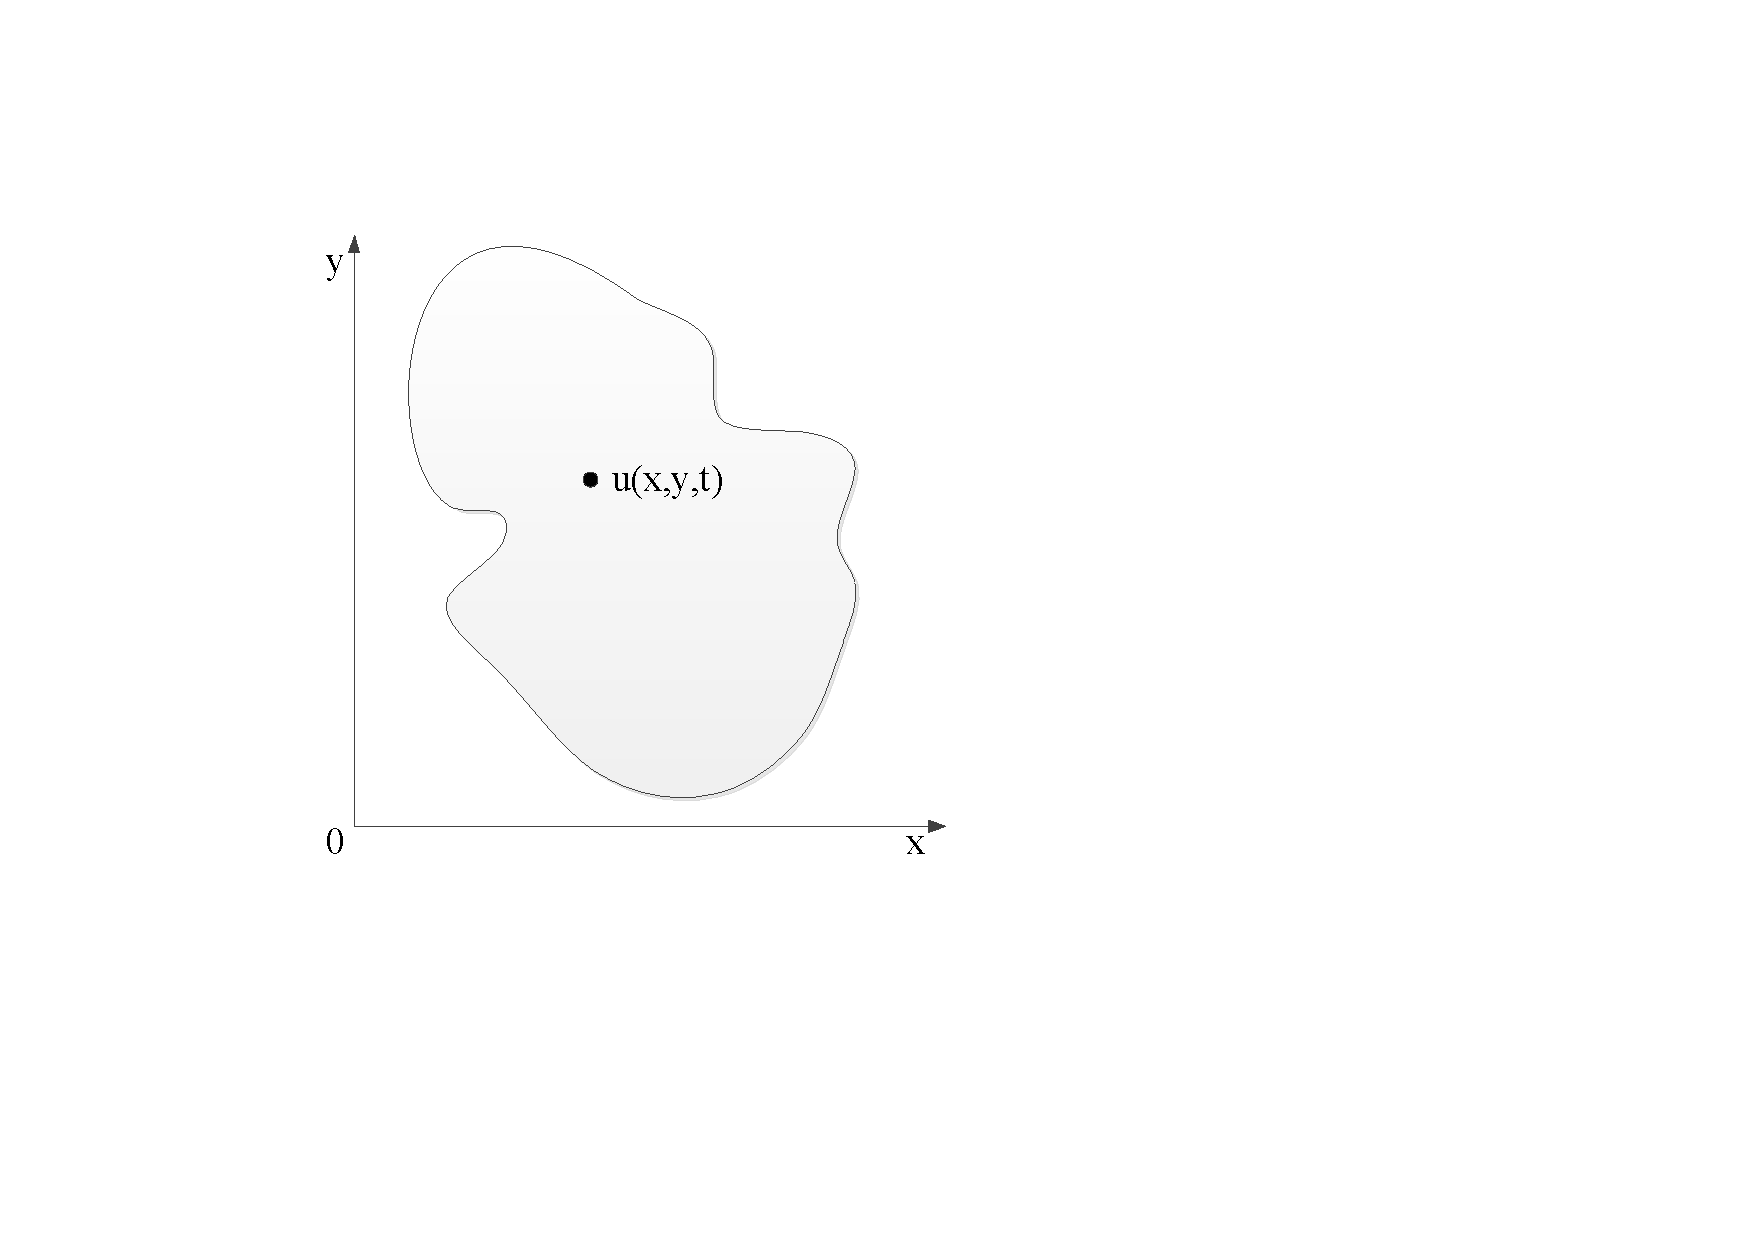
\includegraphics[width=5cm]{fig1.pdf}       
	\caption{System description in 2 dimensions}\label{heatElement.fig}
%COMMENT: do not count yourself: TODO use intensively \label and \ref
\end{figure}

\paragraph{Model}
Consider a small rectangular element of the body with vertices $(x,y)$, $(x+dx,y)$, $(x, y+dy)$, and $(x+dx, y+dy)$. The heat flows are shown in Figure 2.
\begin{figure}[htb]
	\centering
	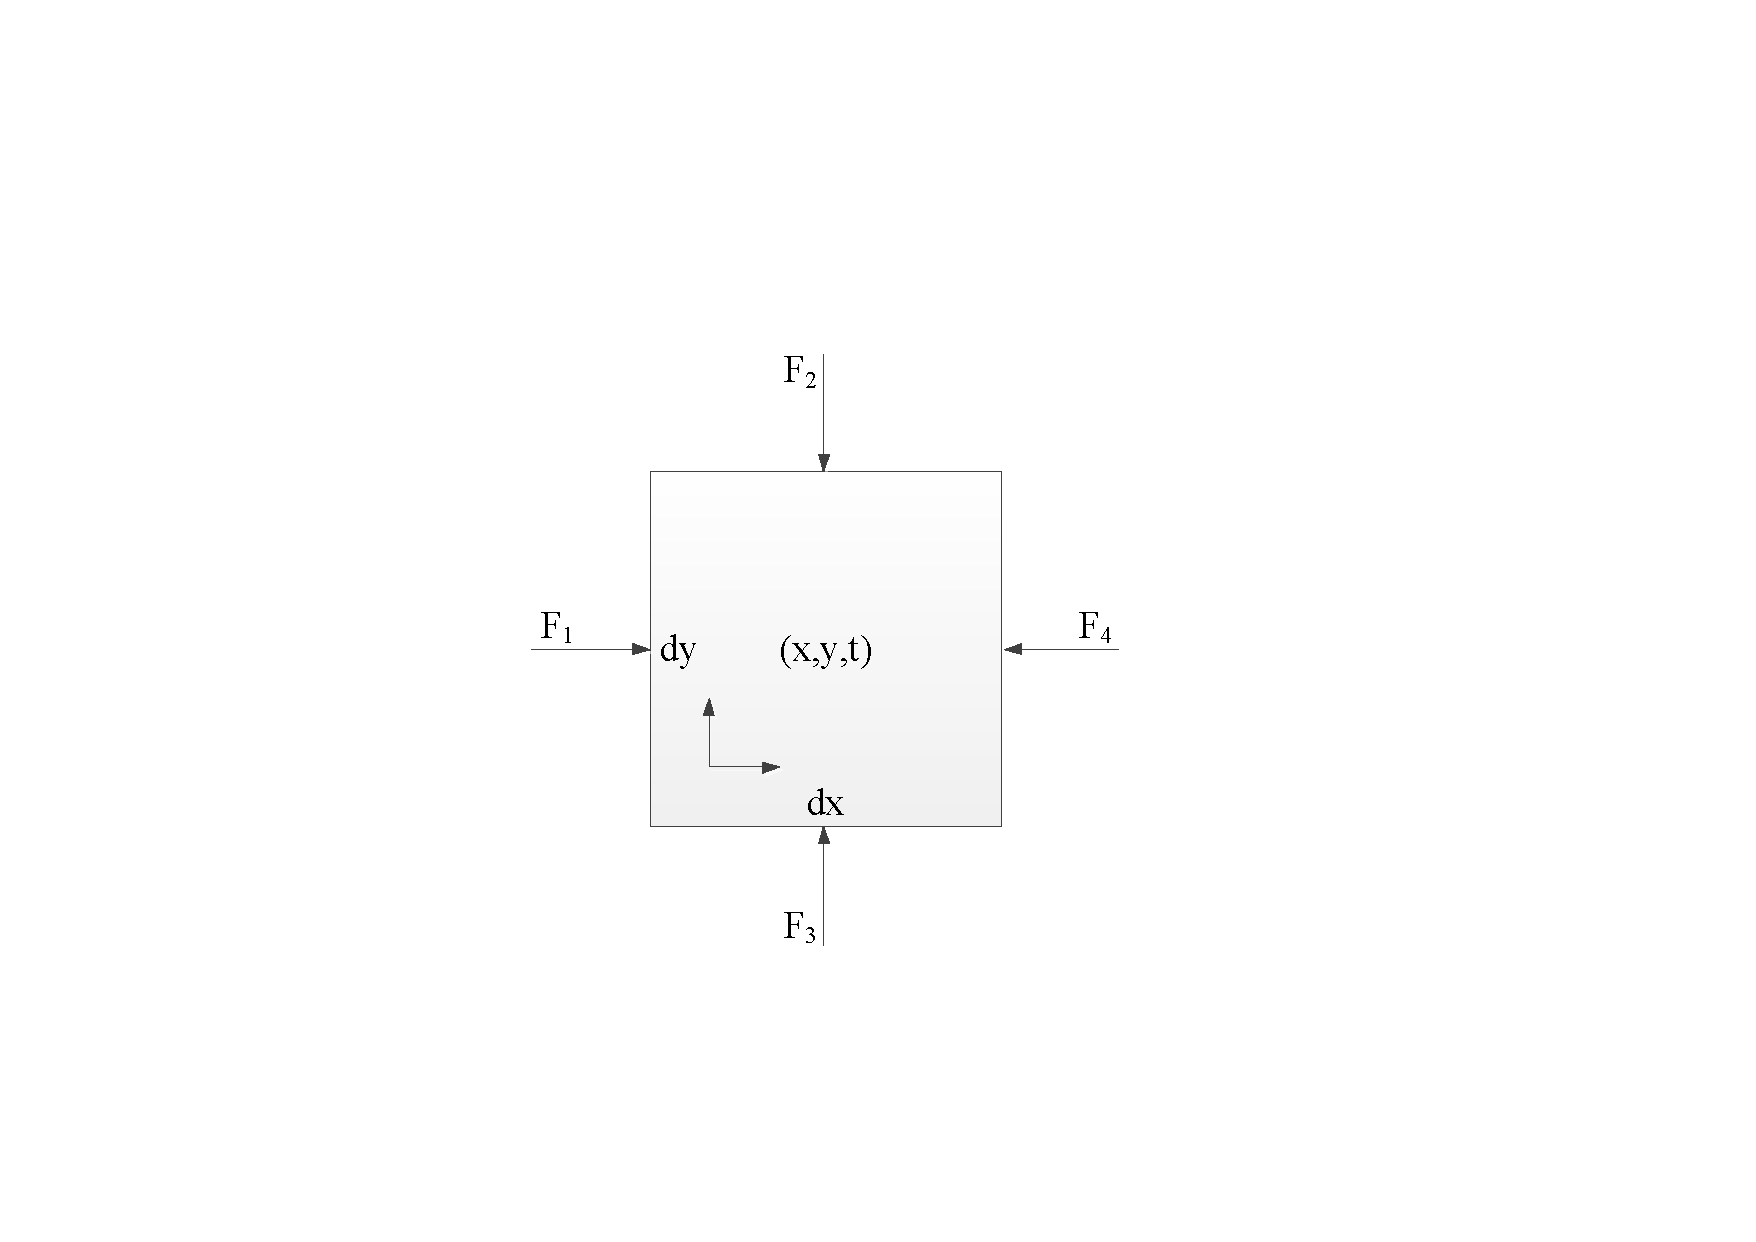
\includegraphics[width=5cm]{fig2.pdf}       
	\caption{Heat flows in a small rectangular element of the body}
\end{figure}

\noindent The heat amount $Q$ (i.e the thermal energy) of the rectangular element at time $t$ is: 
\begin{equation}
Q(x,y,t)=C m T(x,y,t)
\end{equation}
where $C$ is called \emph{heat capacity}, which is a supposed to be constant (assuming the material is uniform and temperature do not vary too much); $m = \rho A$ is the mass of the rectangular element where $A$ its surface.

The rate of thermal energy change with respect to time is therefore:
\begin{equation}\label{thermalEnergyChange.eq}
\frac{\partial Q}{\partial t} = C\rho \ud x \ud y\frac{\partial T}{\partial t}
\end{equation}
As shown in Figure~\ref{heatElement.fig}, the incoming flow is $F_1 + F_2 + F_3 + F_4$. Denote the heat flux $\vec q$ in horizontal and vertical directions by $q_x$ and $q_y$, then we have:
\begin{eqnarray} %COMMENT: the best environment for multiple equation; you can align with & as shown below TODO replace by eqnarray
F_1 &=& q_x(x,y,t)\ud y\label{flow1}\\
F_2 &=& -q_y(x,y+dy,t)dx\label{flow2}\\
F_3 &=& q_y(x,y,t)dx\label{flow3}\\
F_4 &=& -q_x(x+dx,y,t)dy\label{flow4}
\end{eqnarray}
%Sum up $F_1\sim F_4$:
%COMMENT: not very explicit, better this way:
Now, we know that according to energy conservation, the thermal energy variation of any small element (as in Equation~(\ref{thermalEnergyChange.eq})) is equal to the total incoming heat flow.  By putting the partial flows as in Equations~(\ref{flow1})-(\ref{flow4}), this conservation principle yields:
\begin{equation}\label{thermalEnergyChange.eq2}
C\rho \ud x \ud y\frac{\partial T}{\partial t} = dy [q_x(x,y,t)-q_x(x+dx,y,t)]+dxh[q_y(x,y,t)-q_y(x,y+dy,t)]
\end{equation}
%COMMENT: use \emph to emphasize
Now, another physical principle, \emph{Fourier's Law}, states that the heat flow is (negatively) proportional to the gradient of temperature:
\begin{equation}\label{FourierLaw.eq}
\vec q = -k\nabla T
\end{equation}
where $k$ is known as the thermal conductivity of the material (also considered as a constant). Then $q_x$ and $q_y$ are expressed as:
\begin{equation}
\begin{split}
q_x=-k\frac{\partial u}{\partial x}\\
q_y=-k\frac{\partial u}{\partial y}
\end{split}
\end{equation}
%TODO: replace numbers by \ref (with the appropriate \label
Hence, Equation (4) can be written as:
\begin{equation}
\frac{\partial Q}{\partial t}=kdyh[\frac{\partial u(x+dx,y,t)}{\partial x}-\frac{\partial u(x,y,t)}{\partial x}]+kdxh[\frac{\partial u(x,y+dy,t)}{\partial y}-\frac{\partial u(x,y,t)}{\partial y}]
\end{equation}
Combine Equation (2)(7):
\begin{equation}
\frac{\partial u(x,y,t)}{\partial t}=\frac{k}{c\rho}(\frac{\partial ^2 u(x,y,t)}{\partial x^2}+\frac{\partial ^2 u(x,y,t)}{\partial y^2})
\end{equation}
Denote $k/c\rho$ by $a^2$, and the two-dimensional heat equation can be drawn:
\begin{equation}
\frac{\partial u}{\partial t}=a^2\left(\frac{\partial ^2 u}{\partial x^2}+\frac{\partial ^2 u}{\partial y^2}\right)
\end{equation}
%COMMENT: look at the use of \left( and \right) to have nice parentheses



\section{Manipulation of partial differential equations}
%----------------------------------------------------------------------

\subsection{Weak formulation}
% ***********************************************************************************
% Pure LaTeX part to be inserted in a document (be careful of depencies of packages & commands)
% Prepared by XXX and YYY under the supervision of Arnaud de La Fortelle
% Fall 2017
% Derivation of the weak formulation of Dirichlet PDE; subsection of the modeling part
% ***********************************************************************************

\subgroup{3}{???}

\paragraph{Objective}

\paragraph{Demonstration}

\[u=0\\
\Delta u=\partial^2\frac{u}{x^2}+\partial^2\frac{u}{y^2}=0\\
\iint_{D}(\frac{\partial u}{\partial x}-\frac{\partial u}{\partial y})dxdy=\oint_{L}Pdx+Qdy\\
P=-\frac{\partial u}{\partial y},Q=\frac{\partial u}{\partial x}\\
\oint_{L}Pdx+Qdy=\oint_{L}(-\frac{\partial u}{\partial y}dx+\frac{\partial u}{\partial x}dy)=\oint_{L}\nabla u(-dx,dy)
\]

\thispagestyle{empty}
%----------------------------------------------------------------------
\chapter{Simulation}
\label{simulation.chap}
%----------------------------------------------------------------------

\section{Objectives}
%----------------------------------------------------------------------
The objective is to obtain numerical data (often the successive states of the system), to visualize these data, to build meaningful statistics and finally to link the results with theoretical considerations. Best would be to compare simulations with analytical results, but this may prove infeasible and then more analysis is required to compare theory and simulations.

\section{Simulation examples}
%----------------------------------------------------------------------
\subsection{Forward Euler simulation of the 1D heat equation}
% ***********************************************************************************
% Pure LaTeX part to be inserted in a document (be careful of depencies of packages & commands)
% Prepared by XXX and YYY under the supervision of Arnaud de La Fortelle
% Fall 2017
% 1D heat diffusion subsection of the simulation part
% ***********************************************************************************

\subgroup{1}{Lin Yang and Bradley Cage}

\paragraph{Model presentation}
What is the model we want to simulate? What do we want to observe? Which is the state space and the dynamics?

\paragraph{Implementation}
Explain the structure of the code. Do not put necessarily all the code (not more than 100 lines) since some routines (functions) can hide efficiently some unnecessary complexity. Provide a code that run (and explicit librairies and dependencies). Ensure your file name is aligned with this part.

 \paragraph{Results}
 Explain the quantities you are studying (i.e. metrics and statistics). Provide good visualization.
 
\paragraph{Interpretation}
Relate these quantities to the model and to theoretical knowledge of the course.

 \paragraph{Conclusion}
 What have we learned? Is everything aligned (theory and practice)? What was difficult? Provide perspectives.
 


\subsection{1D vibrating string simulation}
% ***********************************************************************************
% Pure LaTeX part to be inserted in a document (be careful of depencies of packages & commands)
% Prepared by XXX and YYY under the supervision of Arnaud de La Fortelle
% Fall 2017
% 1D string waves subsection of the simulation part
% ***********************************************************************************

\subgroup{2}{Qingan Zhao and Ruitong Zhu}

\paragraph{Model presentation}
What is the model we want to simulate? What do we want to observe? Which is the state space and the dynamics?

\paragraph{Implementation}
Explain the structure of the code. Do not put necessarily all the code (not more than 100 lines) since some routines (functions) can hide efficiently some unnecessary complexity. Provide a code that run (and explicit librairies and dependencies). Ensure your file name is aligned with this part.

 \paragraph{Results}
 Explain the quantities you are studying (i.e. metrics and statistics). Provide good visualization.
 
\paragraph{Interpretation}
Relate these quantities to the model and to theoretical knowledge of the course.

 \paragraph{Conclusion}
 What have we learned? Is everything aligned (theory and practice)? What was difficult? Provide perspectives.
 
This code aims to simulate the vibration string (i.e., wave equation) in one dimension. The partial differential equation (PDE) of this problem is given as follow:

\begin{equation}
\frac{\partial^2 h}{\partial t^2}=a^2\left(\frac{\partial^2 h}{\partial x^2}\right)
\end{equation}

where $h$ is the wave function of each point so that the displacement of the string at position $x$ and time $t$ are described as $h(x,t)$; $a$ is the wave speed which equals to $(E/\rho)^{0.5}$.

The simluation is based on finite differences method (FDM). Assume the wave speed $a$ equals to $1$; the length of the string (constrained at both ends) is $2$; the maxium time for this simulation is $4$; stepsize $dx$ and $dt$ are both equal to $0.01$. The initial condition of shape and speed are described as follows:

\begin{eqnarray}
h(x,0)&=&sin(\pi x)\\
\frac{\partial h}{\partial t}\bigg |_{(x,0)}&=&0
\end{eqnarray}

The boundary conditions are described as follows:
\begin{equation}
h(0,t)=h(2,t)=0
\end{equation}

Here is the code:
\begin{python}
	import numpy as np
	import math
	from mpl_toolkits.mplot3d import Axes3D
	from matplotlib import pyplot as plt
	from matplotlib import rc
	plt.rc('text', usetex=True)
	plt.rc('font', family='serif')

	## parameter
	a = 1  ## a coefficient of stiffness
	L = 2  ## The string is constrained at x=0 and x=L.
	T = 4  ## maxium time for this simulation.
	dx = 0.01  ## time step
	dt = 0.01  ## distance step
	N = int(L / dx);
	M = int(T / dt);
	r = (a * dt / dx) ** 2  ## a parameter
\end{python}
	
\begin{python}
	## initial shape of the string
	def initial(x):
	tmp = math.sin(math.pi * x)
	return tmp
	
	## initial speed of the string
	def diff(x):
	tmp = 0 * x
	return tmp
	
	## Define an array and a blank matrix for later use.
	x = [0]
	h = np.zeros((M + 1, N + 1))
	
	## t=0
	for i in range(N):
	x.append(x[i] + dx)  ## x axis
	h[0, i + 1] = initial(x[i + 1])  ## displacement of the string
	
	## t=dt
	for i in range(N - 1):
	h[1, i + 1] = h[0, i + 1] + r * (h[0, i] + h[0, i + 2] - 2 * h[0, i + 1]) / 2 + dx * diff(x[i + 1])
	## displacement of the string
	
	## t=n*dt n>1
	for j in range(1, M):
	for i in range(N - 1):
	h[j + 1, i + 1] = (h[j, i + 2] + h[j, i] - 2 * h[j, i + 1]) * r - h[j - 1, i + 1] + 2 * h[j, i + 1]
	## displacement of the string
	
	t = [0]
	for j in range(M):
	t.append(t[j] + dt)  ## t axis
\end{python}

\bigskip Plot the 3D graph $(x,t,h)$:

\begin{python}
	## Plot the 3D figure.
	fig = plt.figure()
	ax = Axes3D(fig)
	X, T= np.meshgrid(x,t)
	ax.plot_surface(X, T, h, cmap='rainbow')
	plt.title(u'Vibrating String',fontsize=14)
	ax.set_xlabel('X')
	ax.set_ylabel('T')
	ax.set_zlabel('h')
	plt.show()
\end{python}

$\\\\\\$ %make sure the following figure is ahead of the texts

\begin{figure}[htb]
\centering
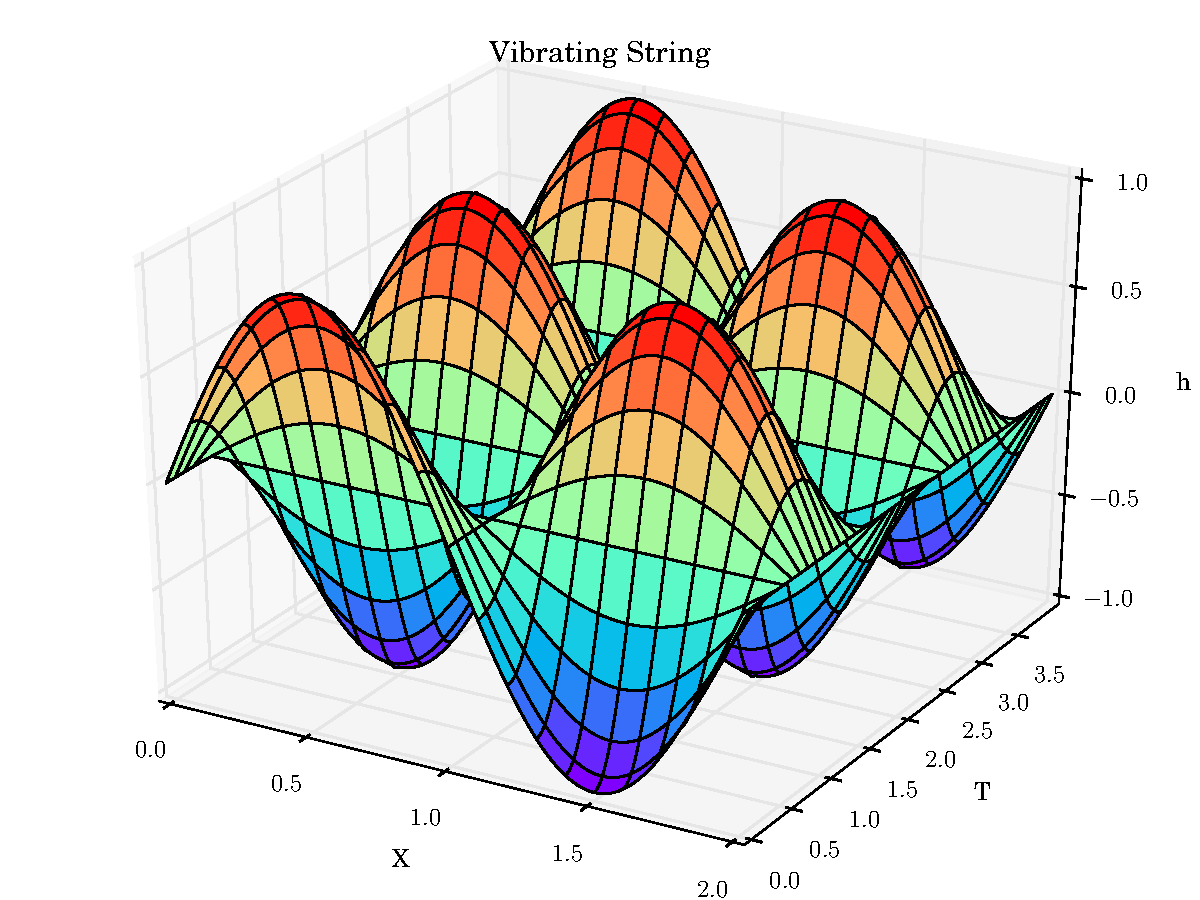
\includegraphics[width=10cm]{3D.pdf}       
\caption{3D graph of the simulation}
\end{figure}

Plot the shape of the string when $t=\{0, 0.5, 1, 1.5, 2\}$:
\begin{python}
	for i in range(5):
	plt.scatter(x,h[i*50,],label="t="+str(i*0.5))
	plt.title(u'Shape of the String',fontsize=14)
	plt.xlabel(u'x',fontsize=14)
	plt.ylabel(u'h',fontsize=14)
	plt.legend(loc='upper left')
	plt.show()
\end{python}

\begin{figure}[htb]
	\centering
	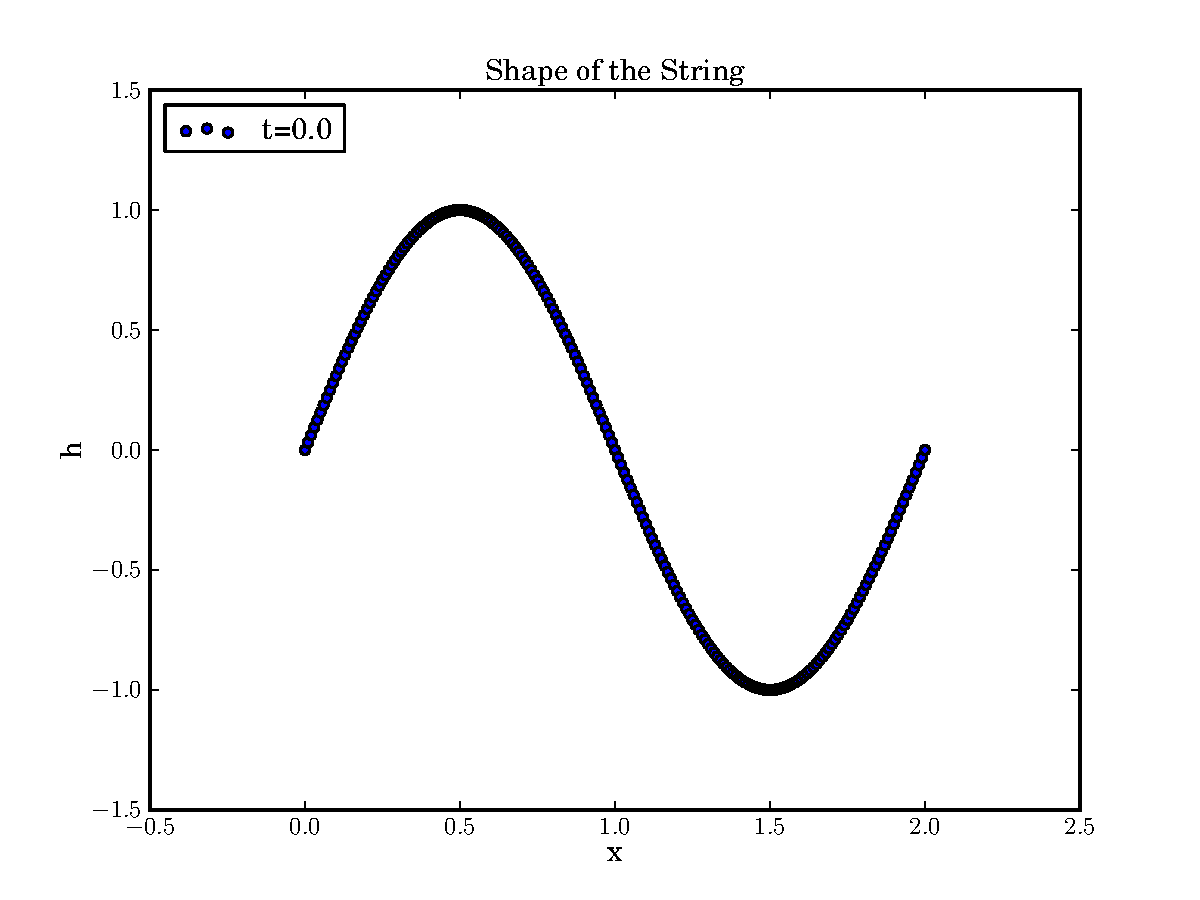
\includegraphics[width=10cm]{t=0.pdf}       
	\caption{Shape of the string when t=0}
\end{figure}

\begin{figure}[htb]
	\centering
	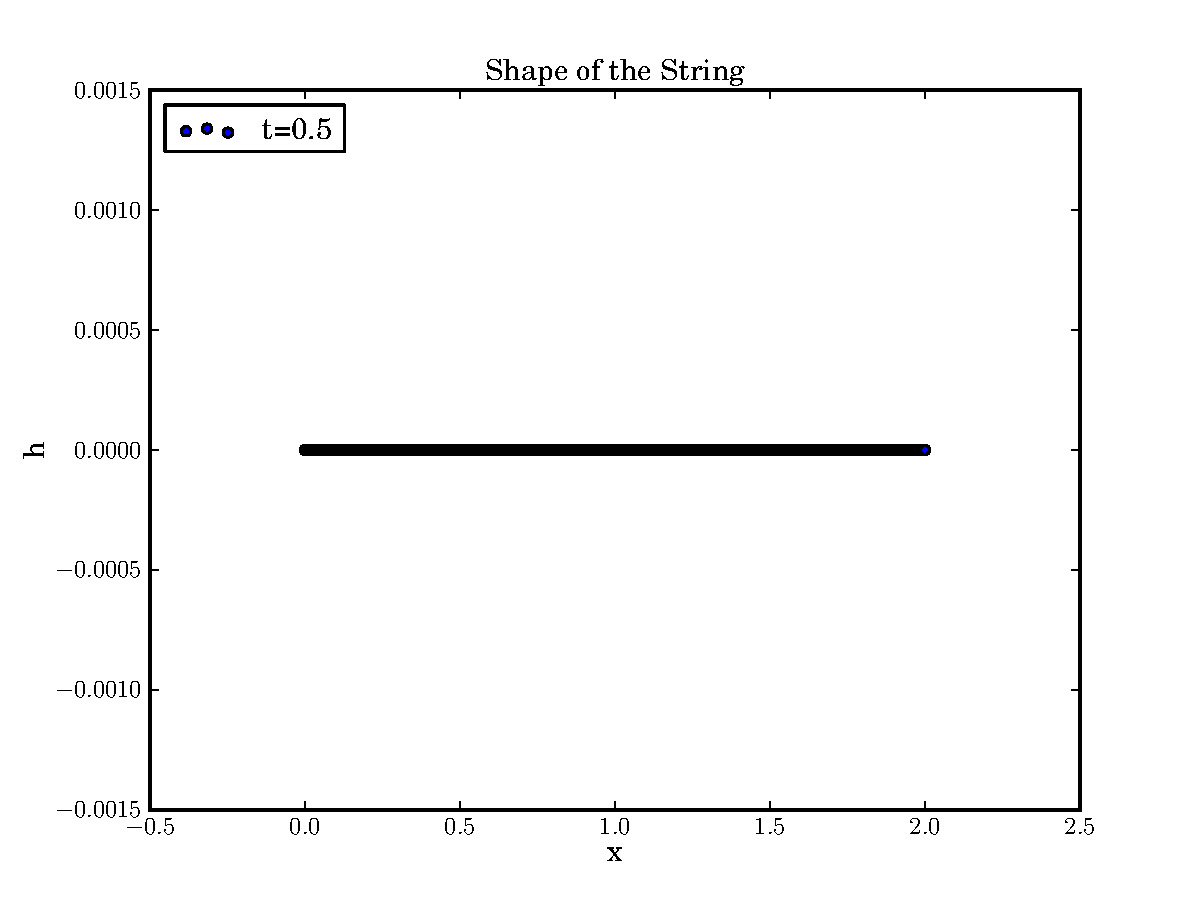
\includegraphics[width=10cm]{t=0_5.pdf}       
	\caption{Shape of the string when t=0.5}
\end{figure}

\begin{figure}[htb]
	\centering
	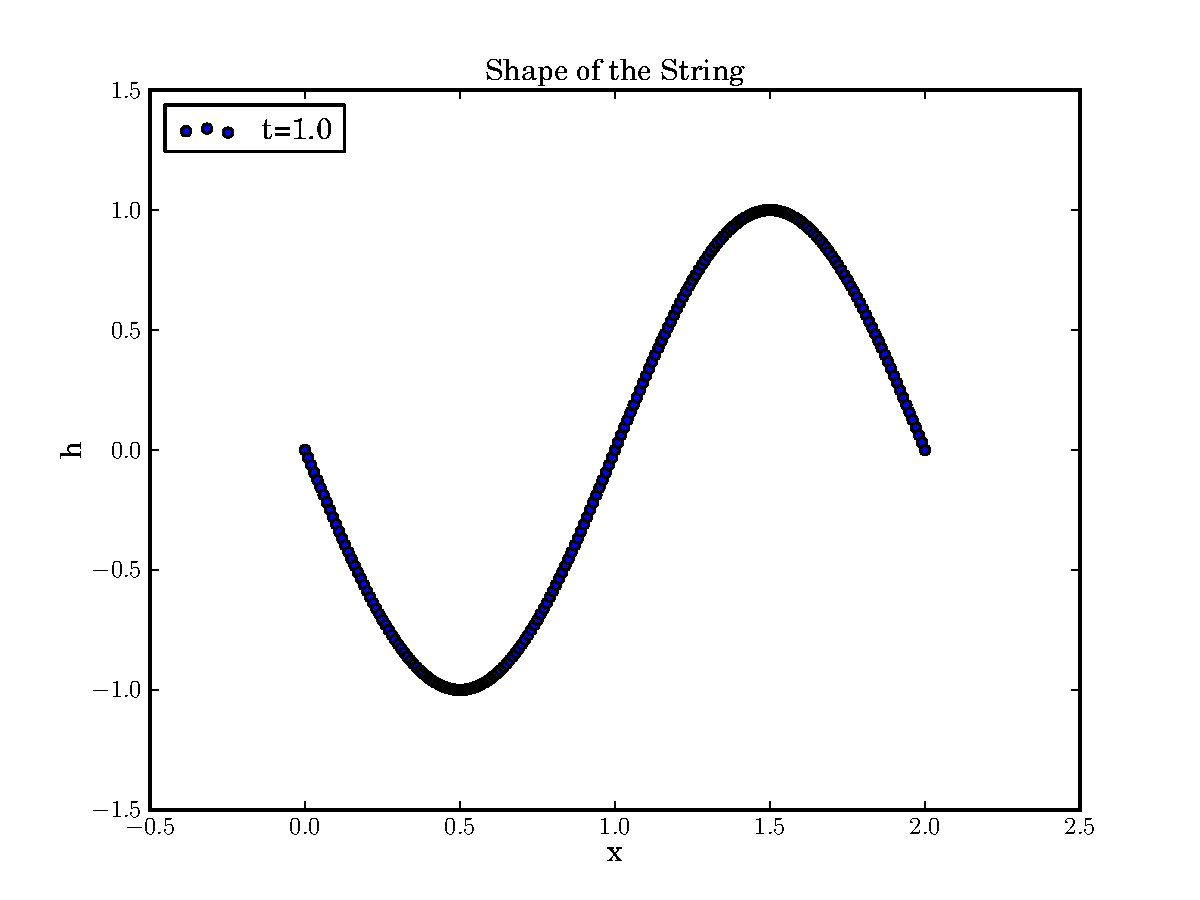
\includegraphics[width=10cm]{t=1.pdf}       
	\caption{Shape of the string when t=1}
\end{figure}

\begin{figure}[htb]
	\centering
	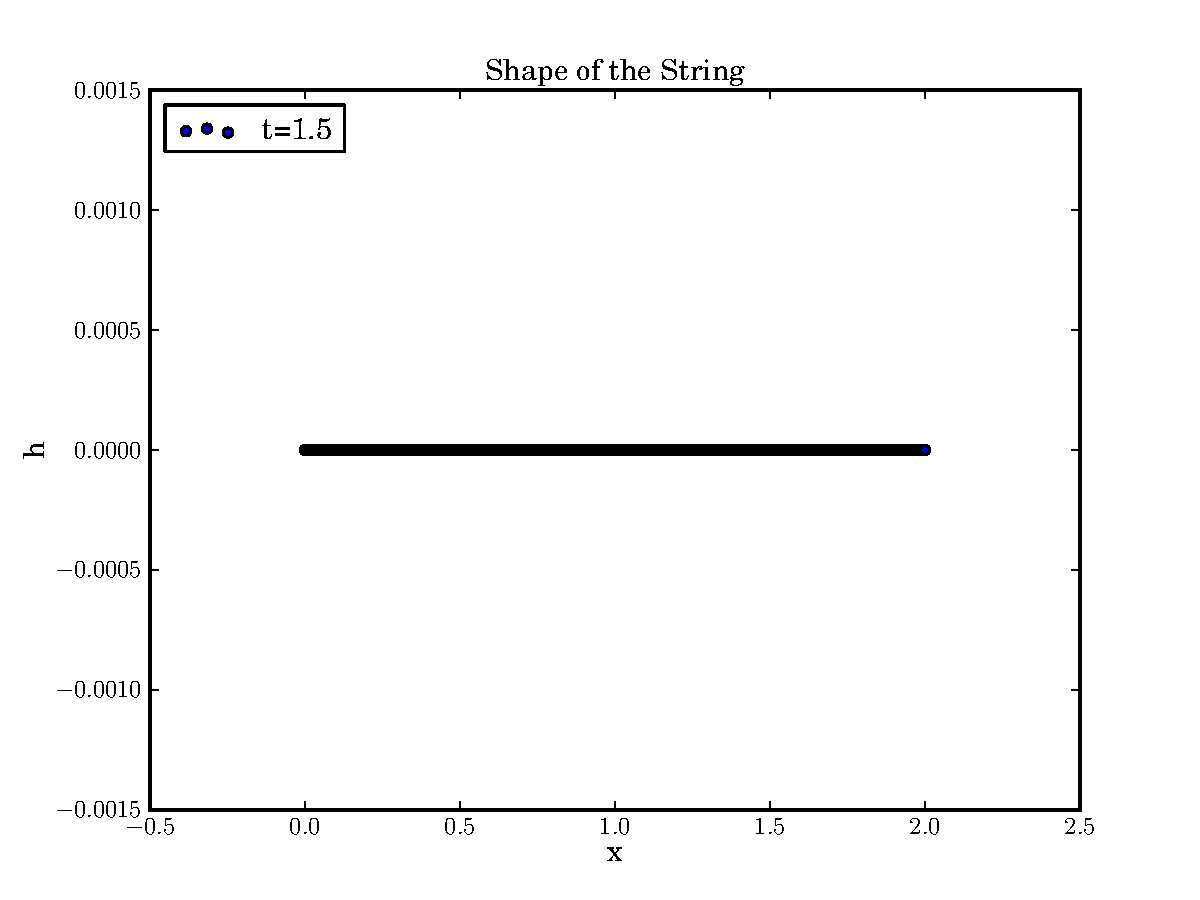
\includegraphics[width=10cm]{t=1_5.pdf}       
	\caption{Shape of the string when t=1.5}
\end{figure}

\begin{figure}[htb]
	\centering
	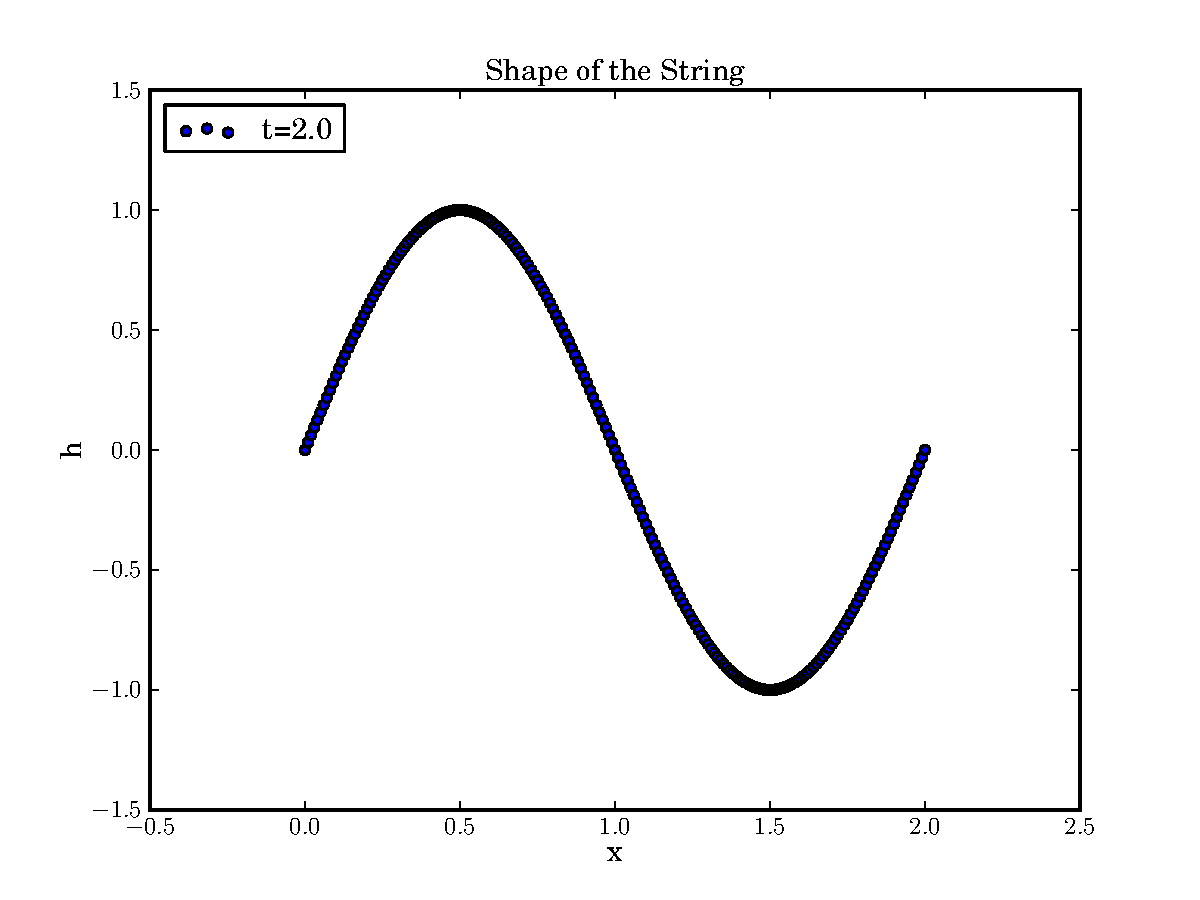
\includegraphics[width=10cm]{t=2.pdf}       
	\caption{Shape of the string when t=2}
\end{figure}


\subsection{1D traffic simulation}
% ***********************************************************************************
% Pure LaTeX part to be inserted in a document (be careful of depencies of packages & commands)
% Prepared by XXX and YYY under the supervision of Arnaud de La Fortelle
% Fall 2017
% 1D LWR traffic model of the simulation part
% ***********************************************************************************

\subgroup{3}{Yue Hu and Carlin Yao}

\paragraph{Model presentation}
What is the model we want to simulate? What do we want to observe? Which is the state space and the dynamics?

\paragraph{Implementation}
Explain the structure of the code. Do not put necessarily all the code (not more than 100 lines) since some routines (functions) can hide efficiently some unnecessary complexity. Provide a code that run (and explicit librairies and dependencies). Ensure your file name is aligned with this part.

 \paragraph{Results}
 Explain the quantities you are studying (i.e. metrics and statistics). Provide good visualization.
 
\paragraph{Interpretation}
Relate these quantities to the model and to theoretical knowledge of the course.

 \paragraph{Conclusion}
 What have we learned? Is everything aligned (theory and practice)? What was difficult? Provide perspectives.
 


\subsection{Random walk in 2D simulation}
% ***********************************************************************************
% Pure LaTeX part to be inserted in a document (be careful of depencies of packages & commands)
% Prepared by XXX and YYY under the supervision of Arnaud de La Fortelle
% Fall 2017
% 12 random walk subsection of the simulation part
% ***********************************************************************************

\subgroup{4}{Yue Hu, Carlin Liao and Robert Ruigrok}

\paragraph{Model presentation}
In this example we simulate the random walk of a particle in a 2D space. A random walk is a mathematical object, known as a stochastic or random process, that describes a path that consists of a succession of random steps. In order to simulate this process, we let a particle move over a discretized grid where its motion is drawn from a set of possible directions. In this simulation we are interested in finding expected distribution of particles after a certain number of time steps as well as the position where they hit the boundaries of the spatial grid.\newline

A particle starts at a specified initial position, from where it begins moving through the grid. In our code, we used a coordinate system to represent the location of a particle as provided in figure \ref{fig:RandomWalkGrid}. The outer border of the grid is enclosed by a ``wall''. When the particle hits this wall, its motion stops and the location where it makes contact is registered.

\begin{figure}[htb]
    \label{fig:RandomWalkGrid}
	\centering
	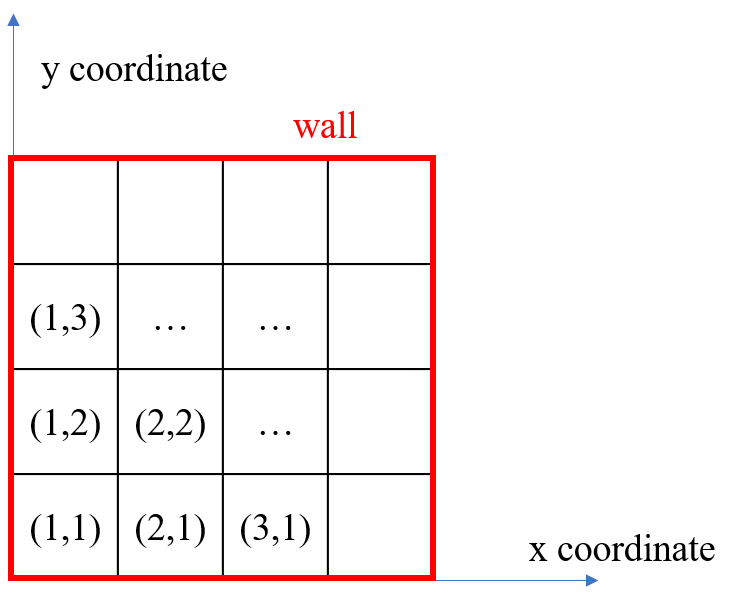
\includegraphics[width=6cm]{RandomWalkGrid.png}       
	\caption{Coordinate representation in spatial grid}
\end{figure}

The dynamics of a particle are relatively straightforward and can be described by equation \ref{eq:RandomWalkDynamics}. A particle has 5 options for its motion: moving up, right, down, left or no motion (options are depicted in figure \ref{fig:RandomWalkMotion}). Every motion has a certain probability $p$ to occur. These probabilities can be given as input and must add up to 1.

\begin{equation}
\label{eq:RandomWalkDynamics}
X_{k+1}(x,y) = X_k(x,y) +  \begin{cases}
(0,1) &\text{with probability $p\uparrow$}\\
(1,0) &\text{with probability $p\rightarrow$}\\
(0,-1) &\text{with probability $p\downarrow$}\\
(-1,0) &\text{with probability $p\leftarrow$}\\
(0,0) &\text{with probability $p\ \bullet$}
\end{cases}
\end{equation}



\begin{figure}[htb]
    \label{fig:RandomWalkMotion}
	\centering
	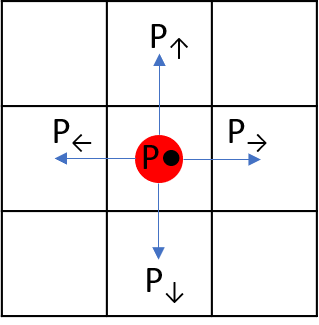
\includegraphics[width=3cm]{RandomWalkMotion.png}       
	\caption{Potential motion per time step}
\end{figure}


\paragraph{Implementation} 
At the top of the file, it is possible to set the grid size, starting position of particles, \# of particles, simulation horizon and motion direction probabilities. The script will also generate snapshots of the particle distribution at different moments in time during the simulation. By selecting the number of subplots, you can determine how many instances you would like to see. This will provide insights into how the particle distribution develops over time. \newline

Particles are simulated one at a time. The simulation runs until the time horizon $T$ is reached or the particle hits the wall. Their position is saved in a 3-dimensional array (time, x-position, y-position) at specified moments in time only; this way the amount of required memory is kept to a minimum. %You do not save the position of every particle at every time step, but you only ``count'' their positions at time steps that you are interested in. Information about individual particles gets lost, but that is fine.
\newline

Information about where particles hit the wall is included in the same arrays. This data ``circumvents'' the $n \times n$ data about the particle distribution within the grid. As a result, when we plot the full array we can see the distribution of particles in the grid at their respective location, and the distribution of particles at the wall directly ``behind'' the wall.\newline

\begin{python}
# This file will model/simulate the random motion

import numpy as np
import matplotlib.pyplot as plt
from random import *
import pylab

############## START INPUT #################

GridSizeSquare = 20 # n, will create an nxn grid
#define starting position as ratio or grid size
Pos_init = np.ceil(np.array([0.4,0.4])*GridSizeSquare)
#T is the total amount of time steps, scale with square of grid size. 0.3 is nice
T = 0.3*np.power(GridSizeSquare, 2)
n_particles = 10000 # #particles. 10000+ recommended
# define the # of subplots for intermediate time snap shots
subplot_row = 2             
subplot_column = 2
#defines the drift probabilities: ([up,right,down,left,0]) 
motion_prob = np.array([0.2,0.2,0.2,0.2,0.2])

############## END INPUT #################

#only look at square grids, but this could be changed:
x_grid = GridSizeSquare
y_grid = GridSizeSquare
n_subplot = subplot_row*subplot_column
Plot_interval = np.floor((T-1)/(n_subplot-1))
#This determines when you take snapshots of the process, every "Plot_interval" time steps

# now define the probabilities of the random walk
# notation of motion ([up,right,down,left,no motion])
# I normalized in case probabilities do not add up to 1...
motion_prob = motion_prob/np.sum(motion_prob)
# define the change in coordinates of every motion:
motion_xy = np.array([[0,1],[1,0],[0,-1],[-1,0],[0,0],])
motion_prob_percentile = np.cumsum(motion_prob)
# this is used later to draw from with randomizer

# make an empty data grid from where you are going to count the amount occurrences and hits against the wall
Data = np.zeros((x_grid+2,y_grid+2)) # "+2" for wall data
Data_resized = np.zeros((Data.shape[0]+1,Data.shape[1]+1))
# This for plotting purposes, I need to add an extra row an column for some reason
# Now create a new empty data set for the intermediate plots:
Data_TimeVarying = np.zeros((n_subplot,Data_resized.shape[0],Data_resized.shape[1]))

# construct some arrays for plotting later on:
xx, yy = pylab.meshgrid(
    pylab.linspace(-1,x_grid+1,x_grid+3),
    pylab.linspace(-1,y_grid+1,y_grid+3))

# Here, start loop over all the particles after each other:
for i in range(1, n_particles+1):
    # Initialize simulation
    t = 0
    HitWall = False
    Pos = Pos_init
    Subplot = 1
    
    # start simulation
    while t < T and not HitWall:
                
         # Now continue with the motion simulation
        MotionRandom = random()
        IndexMotion = np.argmax(motion_prob_percentile>MotionRandom)
        Pos = Pos + motion_xy[IndexMotion,:] #this works
        
        # Now check for hitting the wall
        if Pos[0] == 0 or Pos[1] == 0 or Pos[0] == x_grid+1 or Pos[1] == y_grid+1:
            if Subplot <= n_subplot:             
                Data_TimeVarying[Subplot-1,Pos[0],Pos[1]] = Data_TimeVarying[Subplot-1,Pos[0],Pos[1]]+1
            HitWall = True

        # Now record the position for time dependent plotting purposes
        if t % Plot_interval == 0 and Subplot <= n_subplot and not(HitWall):   #so create a subplot every Plot_interval time steps
            Data_TimeVarying[Subplot-1,Pos[0],Pos[1]] = Data_TimeVarying[Subplot-1,Pos[0],Pos[1]]+1
            Subplot = Subplot+1        
        
        t = t+1
    
    
    #This was basically the whole simulation, now save the results
    Data[Pos[0],Pos[1]] = Data[Pos[0],Pos[1]] + 1
    # I need to give resize Data with an extra row and column, since pcolor doesn't plot the full range of the matrix...
    Data_resized[:-1,:-1] = Data       


# Now I need to do some post-processing of the intermediate measurements.
# I need to add the particles that hit the wall in earlier time steps to the 
# later plots, so the total amount of particles is always n  
Data_TimeVarying_Corrected = np.cumsum(Data_TimeVarying,axis=0)
Data_TimeVarying_Corrected[:,1:x_grid+1,1:y_grid+1] = Data_TimeVarying[:,1:x_grid+1,1:y_grid+1]


# This loop creates subplots at several time instances
plt.figure()
for j in range(1, n_subplot+1):
    #Now visualize the outcomes
    pylab.subplot(subplot_row, subplot_column, j)
    pylab.pcolor(xx,yy,np.transpose(Data_TimeVarying_Corrected[j-1,:,:]))
    TitleString = 'Distribution at t = ' + str((j-1)*Plot_interval+1)
    pylab.title(TitleString)
    # and a color bar to show the correspondence between function value and color
    pylab.colorbar()
    pylab.hold(True)
    pylab.plot([0, x_grid],[0, 0], 'r',[0, x_grid],[y_grid, y_grid], 'r',[0, 0],[0, y_grid], 'r',[x_grid, x_grid],[0, y_grid], 'r')
    pylab.plot(Pos_init[0]-0.5,Pos_init[1]-0.5,'ro')

pylab.show()

# This plot shows the final distribution, including distribution along the walls
plt.figure()
pylab.pcolor(xx,yy,np.transpose(Data_resized))
pylab.title('Final distribution at t = %d, including hitting walls' %T)
# and a color bar to show the correspondence between function value and color
pylab.colorbar()
pylab.hold(True)
pylab.plot([0, x_grid],[0, 0], 'r',[0, x_grid],[y_grid, y_grid], 'r',[0, 0],[0, y_grid], 'r',[x_grid, x_grid],[0, y_grid], 'r')
pylab.plot(Pos_init[0]-0.5,Pos_init[1]-0.5,'ro')
pylab.show
\end{python}



\paragraph{Results}
In this section we included two simulation for both a $10x10$ grid and a $20 \times 20$ grid, with a different simulation time horizon $T$. Both simulations use 10,000 particles and have a motion probability of $0.2$ in all directions. \newline

It is clearly visible how the particles spread out over time and make their way to the walls over time. The more particles that are simulated per grid resolution, the smoother the distribution becomes. You can clearly see that 10,000 particles simulated lead to a clean distribution in the smaller plot of figure \ref{fig:RandomWalk10}, while the larger plot of \ref{fig:RandomWalk20} shows a more grainy distribution.

\begin{figure}[htb]
    \label{fig:RandomWalk10}
	\centering
	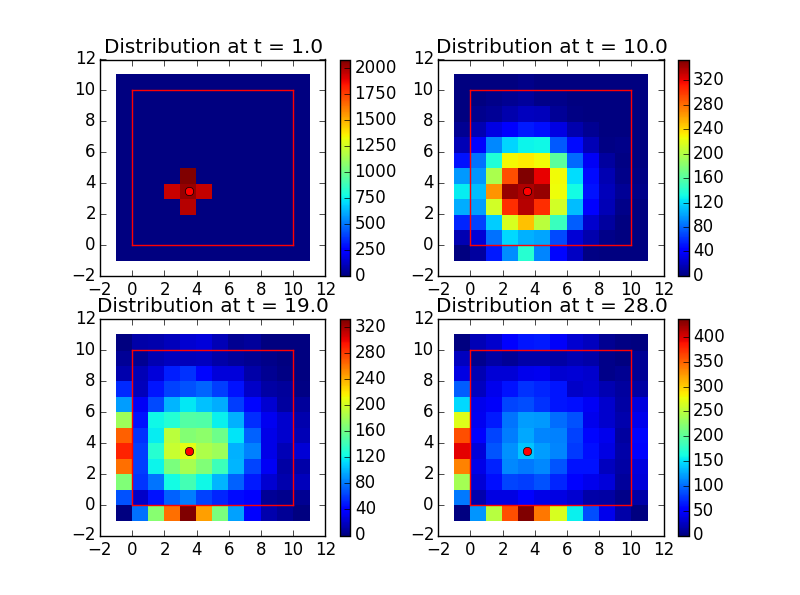
\includegraphics[width=14cm]{figure10x10.png}       
	\caption{Particle distribution for $10 \times 10$ grid at different time steps}
\end{figure}

\begin{figure}[htb]
    \label{fig:RandomWalk20}
	\centering
	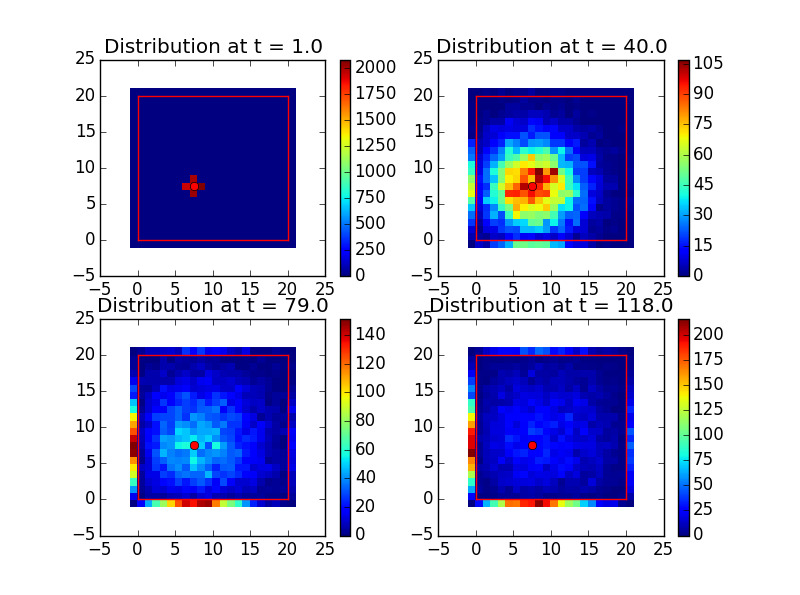
\includegraphics[width=14cm]{figure20x20.png}       
	\caption{Particle distribution for $20 \times 20$ grid at different time steps}
\end{figure}


 
\paragraph{Interpretation}
{\it Relate these quantities to the model and to theoretical knowledge of the course.}\newline

{\it I think this motion is described by Fick's Law in 2 dimension. The concentration on a specific point changes over time, depending on the concentration of its surroundings. Should we derive why the second derivative matters? $\phi$ is the concentration, $D$ the diffusion coefficient.}

\begin{equation}
\label{eq:FicksLaw}
\frac{d\phi}{dt} = D\nabla\phi = D \big(\frac{d^2\phi}{dx^2} + \frac{d^2\phi}{dy^2}\big)
\end{equation}


 \paragraph{Conclusion}
 \textit{What have we learned? Is everything aligned (theory and practice)? What was difficult? Provide perspectives.}
 
 The dynamics of the random walk were easy to model. The challenge in this simulation was to save the data for the intermediate time steps. Since the particles are simulated one by one for the full time horizon, we had to write some non-intuitive code to save the location of every particle at the relevant intermediate time steps. \newline
 
 From the lecture we recall that diffusion distance scales with the square root of time. Here we tried to simulate that. When doubling the grid size and taking a four times higher simulation horizon, the distribution looks similar. However, we have the idea that the scaling did not work for 100\%. At the end of the scaled simulation horizon, it seems as if the smaller grid has relatively more particles in the grid than the larger grid has. What could cause this difference?
 

\thispagestyle{empty}
%----------------------------------------------------------------------
\chapter{Control}
\label{control.chap}
%----------------------------------------------------------------------

\section{Objectives}
%----------------------------------------------------------------------




\end{document}



